\documentclass[12pt,a4paper]{article}

% ============================================================
% PACKAGES
% ============================================================
\usepackage[left=1in,right=1in,top=1in,bottom=1in]{geometry}
\usepackage{graphicx}
\usepackage{booktabs}
\usepackage{array}
\usepackage{tabularx}
\usepackage{colortbl}
\usepackage{xcolor}
\usepackage{makecell}
\usepackage{fancyhdr}
\usepackage{titlesec}
\usepackage{amsmath}
\usepackage{tcolorbox}
\usepackage{listings}
\usepackage{float}

\definecolor{codebg}{RGB}{232,238,246}

\tcbset{
    colback=white,
    colframe=blue!40!black,
    boxrule=0.4pt,
    arc=2pt,
    leftrule=2.5pt,
    left=6pt,
    right=6pt,
    top=6pt,
    bottom=4pt,
}

\lstset{
    basicstyle=\ttfamily\scriptsize,
    backgroundcolor=\color{codebg},
    breaklines=true,
    breakatwhitespace=false,
    columns=fullflexible,
    keepspaces=true,
    aboveskip=6pt,
    belowskip=2pt,
    frame=none,
    xleftmargin=0pt,
    xrightmargin=0pt,
    language=Python,
}

\definecolor{headerblue}{RGB}{213,220,228}

\newcolumntype{Y}{>{\centering\arraybackslash}X}
\newcolumntype{L}{>{\raggedright\arraybackslash}X}

\setlength{\parindent}{0pt}
\setlength{\parskip}{6pt}

\pagestyle{fancy}
\fancyhf{}
\rhead{SE: Machine Learning Lab}
\lhead{Lab 8}
\rfoot{\thepage}

\begin{document}

% ============================================================
% HEADER
% ============================================================
\renewcommand{\arraystretch}{2.0}
\begin{tabularx}{\textwidth}{|Y|}
\hline
\rowcolor{headerblue} \textbf{\large Department of Computer and Software Engineering} \\
\hline
\textbf{\large SE: Machine Learning} \\
\hline
\end{tabularx}
\renewcommand{\arraystretch}{1.0}

\vspace{12pt}

% ============================================================
% COURSE INFO
% ============================================================
\renewcommand{\arraystretch}{2.0}
\begin{tabularx}{\textwidth}{|L|L|}
\hline
\textbf{Course Instructor:} & \textbf{Date:} \\
\hline
\textbf{Day:} & \textbf{Semester:} \\
\hline
\end{tabularx}
\renewcommand{\arraystretch}{1.0}

\vspace{12pt}

% ============================================================
% TITLE
% ============================================================
\begin{center}
{\Large\bfseries Lab 8: Fraud Detection using Isolation Forest and Gaussian Density}
\end{center}

\vspace{6pt}

% ============================================================
% META TABLE
% ============================================================
\renewcommand{\arraystretch}{1.8}
\begin{tabularx}{\textwidth}{|Y|c|c|c|c|}
\hline
\textbf{Lab Title} & \textbf{CLO} & \textbf{BT} & \textbf{PLO} & \textbf{Weightage} \\
\hline
\makecell{{\small Fraud Detection} \\ {\small using Isolation Forest and Gaussian Density}} & & & & \\
\hline
\end{tabularx}
\renewcommand{\arraystretch}{1.0}

\vspace{6pt}

% ============================================================
% STUDENT TABLE
% ============================================================
\renewcommand{\arraystretch}{2.0}
\begin{tabularx}{\textwidth}{|Y|Y|Y|Y|Y|}
\hline
\textbf{Name} & \textbf{Roll Number} & \textbf{Report /10} & \textbf{Viva /5} & \textbf{Total /15} \\
\hline
Muhammad Abdul Qadir & BSSE23105 & & & \\
\hline
\end{tabularx}
\renewcommand{\arraystretch}{1.0}

\vspace{12pt}

\begin{flushright}
Checked on: \_\_\_\_\_\_\_\_\_\_\_\_\_\_\_\_

\vspace{6pt}

Signature: \_\_\_\_\_\_\_\_\_\_\_\_\_\_\_\_
\end{flushright}

\newpage

% ============================================================
% OBJECTIVES
% ============================================================

\section*{Objectives}

\begin{itemize}
\item Understand anomaly detection in real-world fraud scenarios
\item Implement Isolation Forest using sklearn
\item Implement Gaussian density estimation from scratch
\item Visualize anomalous regions
\end{itemize}

% ============================================================
% PROBLEM STATEMENT
% ============================================================

\section*{Problem Statement}

You are designing a fraud detection system for a bank. Each transaction is represented using two features:

\begin{itemize}
\item Transaction Amount
\item Time Gap Since Last Transaction
\end{itemize}

Normal transactions follow consistent patterns, while fraudulent transactions tend to deviate significantly.

Your task is to detect fraudulent transactions using:

\begin{itemize}
\item Isolation Forest (algorithmic approach)
\item Gaussian Density Estimation (probabilistic approach)
\end{itemize}

% ============================================================
% DATASET
% ============================================================

\section*{Dataset Description}

A synthetic dataset is provided:

\begin{itemize}
\item Normal data: Gaussian distribution
\item Fraud data: Random outliers
\item Labels:
    \begin{itemize}
    \item 1 = Normal
    \item -1 = Fraud
    \end{itemize}
\end{itemize}

% ============================================================
% TASKS
% ============================================================

\section*{Part A: Isolation Forest (9 Marks)}

\begin{tcolorbox}
\textbf{Task 1: Train Isolation Forest}

Implement a function to train an Isolation Forest model on the given dataset. 
The model isolates anomalies by recursively splitting the data using random 
feature selection and split values.

\begin{lstlisting}
def fit_isolation_forest(X):
    my_isolation_forest_anomaly_model = IsolationForest(
        random_state=42
    )
    my_isolation_forest_anomaly_model.fit(X)
    return my_isolation_forest_anomaly_model
\end{lstlisting}

\textbf{Output:} Fitted on 310 samples with default settings (100 trees, auto contamination). The model is now ready to flag outliers.

\end{tcolorbox}

\vspace{14pt}

\begin{tcolorbox}
\textbf{Task 2: Predict Anomalies}

Use the trained model to classify each transaction as normal or anomalous. 
Observe how many points are identified as anomalies and compare with the 
actual distribution.

\begin{lstlisting}
def predict_iforest(model, X):
    predicted_labels_from_isolation_forest = model.predict(X)
    return predicted_labels_from_isolation_forest
\end{lstlisting}

\textbf{Output:}
\begin{itemize}
\item Total samples processed: 310
\item Transactions classified as normal: 269
\item Transactions flagged as anomalous: 41
\item Ground truth fraud count: 30
\end{itemize}

Out of 310 transactions, 41 were flagged while 30 are actually fraudulent. The extra 11 are false alarms from borderline normal transactions.

\end{tcolorbox}

\vspace{14pt}

\begin{tcolorbox}
\textbf{Task 3: Analyze Anomaly Scores}

Compute anomaly scores for all data points. These scores are related to 
the path length required to isolate a point in the trees. Points that are 
isolated quickly (short path length) are more likely to be anomalies.

\begin{lstlisting}
def compute_iforest_scores(model, X):
    computed_anomaly_scores_for_each_point = (
        model.decision_function(X)
    )
    return computed_anomaly_scores_for_each_point
\end{lstlisting}

\textbf{Output:}
\begin{itemize}
\item Score range: $-0.2355$ to $0.1281$
\item Negative scores indicate normal-looking data points
\item Positive scores indicate more suspicious transactions
\end{itemize}

Negative scores mean the point blends in with normal data, while positive scores mean it was easy to isolate and likely anomalous.

\end{tcolorbox}

% ============================================================

\section*{Part B: Gaussian Density Estimation (12 Marks)}

\begin{tcolorbox}
\textbf{Task 4: Estimate Gaussian Parameters}

Compute the mean and covariance matrix of the dataset.

\[
\mu = \frac{1}{N} \sum_{i=1}^{N} x_i
\]

\[
\Sigma = \frac{1}{N} \sum_{i=1}^{N} (x_i - \mu)(x_i - \mu)^T
\]

These parameters represent the center and spread of the data.

\begin{lstlisting}
def compute_gaussian_params(X):
    calculated_mean_vector_of_dataset = np.mean(X, axis=0)
    calculated_covariance_matrix_of_dataset = np.cov(
        X, rowvar=False
    )
    return (calculated_mean_vector_of_dataset,
            calculated_covariance_matrix_of_dataset)
\end{lstlisting}

\textbf{Output:}

\vspace{4pt}
Mean: $\mu = [50.2925,\ 33.0601]$

\vspace{4pt}
Covariance matrix:
\[
\Sigma = \begin{bmatrix} 181.6055 & 5.5934 \\ 5.5934 & 181.1962 \end{bmatrix}
\]

The center of the data sits around (50, 33). Both features have similar variance ($\approx$181) and the small off-diagonal values show they are nearly independent.

\end{tcolorbox}

\vspace{14pt}

\begin{tcolorbox}
\textbf{Task 5: Compute Probability Density}

Compute the probability density of each data point using the multivariate 
Gaussian distribution:

\[
p(x) = \frac{1}{(2\pi)^{d/2} |\Sigma|^{1/2}} 
\exp\left(-\frac{1}{2}(x-\mu)^T \Sigma^{-1} (x-\mu)\right)
\]

Points far from the mean will have lower probability values.

\begin{lstlisting}
def gaussian_density(X, mu, sigma):
    num_features = X.shape[1]
    det_sigma = np.linalg.det(sigma)
    inv_sigma = np.linalg.inv(sigma)
    
    norm_const = 1.0 / (
        ((2 * np.pi) ** (num_features / 2.0))
        * (det_sigma ** 0.5)
    )
    
    densities = np.zeros(X.shape[0])
    for i in range(X.shape[0]):
        diff = X[i] - mu
        exp_val = -0.5 * np.dot(
            np.dot(diff.T, inv_sigma), diff
        )
        densities[i] = norm_const * np.exp(exp_val)
        
    return densities
\end{lstlisting}

\textbf{Output:}
\begin{itemize}
\item Minimum density observed: $5.4315 \times 10^{-10}$
\item Maximum density observed: $8.7766 \times 10^{-4}$
\end{itemize}

Densities range across six orders of magnitude --- central points sit around $10^{-4}$ while outliers drop to $10^{-10}$. This wide gap makes it easy to separate normal from fraudulent.

\end{tcolorbox}

\vspace{14pt}

\begin{tcolorbox}
\textbf{Task 6: Detect Anomalies using Threshold}

Classify transactions based on probability values:

\[
\text{If } p(x) < \epsilon \Rightarrow \text{Anomaly}
\]

\[
\text{Else } \Rightarrow \text{Normal}
\]

Experiment with different values of $\epsilon$ and observe how the classification changes.

\begin{lstlisting}
def predict_gaussian(X, mu, sigma, threshold):
    probs = gaussian_density(X, mu, sigma)
    predictions = np.ones(X.shape[0])
    predictions[probs < threshold] = -1
    return predictions
\end{lstlisting}

\textbf{Output} (using 5th percentile as $\epsilon = 2.3485 \times 10^{-6}$):
\begin{itemize}
\item Predicted normal: 294
\item Predicted anomaly: 16
\end{itemize}

\vspace{6pt}

\textbf{Exploring how different $\epsilon$ values affect detection:}

\begin{center}
\begin{tabular}{|c|c|c|}
\hline
\textbf{$\epsilon$} & \textbf{Normal} & \textbf{Anomaly} \\
\hline
$10^{-7}$ & 301 & 9 \\
\hline
$10^{-6}$ & 298 & 12 \\
\hline
$10^{-5}$ & 291 & 19 \\
\hline
$10^{-4}$ & 283 & 27 \\
\hline
$10^{-3}$ & 0 & 310 \\
\hline
$10^{-2}$ & 0 & 310 \\
\hline
\end{tabular}
\end{center}

With small $\epsilon$ values ($10^{-7}$), we only catch the worst outliers. As $\epsilon$ grows, more cases get flagged --- 27 out of 30 real frauds at $10^{-4}$. Past $10^{-3}$, everything gets marked as anomalous. So $10^{-5}$ to $10^{-4}$ is the practical sweet spot for this data.

\end{tcolorbox}

% ============================================================

\section*{Part C: Visualization (6 Marks)}

\begin{tcolorbox}
\textbf{Task 7: Visualize Dataset}

Plot the dataset in a two-dimensional space. Clearly distinguish between 
normal and anomalous transactions using different colors.

\begin{lstlisting}
def plot_points(X, labels, title):
    color_list = [
        'blue' if lbl == 1 else 'red' for lbl in labels
    ]
    plt.scatter(
        X[:,0], X[:,1], c=color_list,
        edgecolors='white', linewidth=0.8, s=40
    )
    plt.title(title)
\end{lstlisting}
\end{tcolorbox}

\begin{figure}[H]
\centering
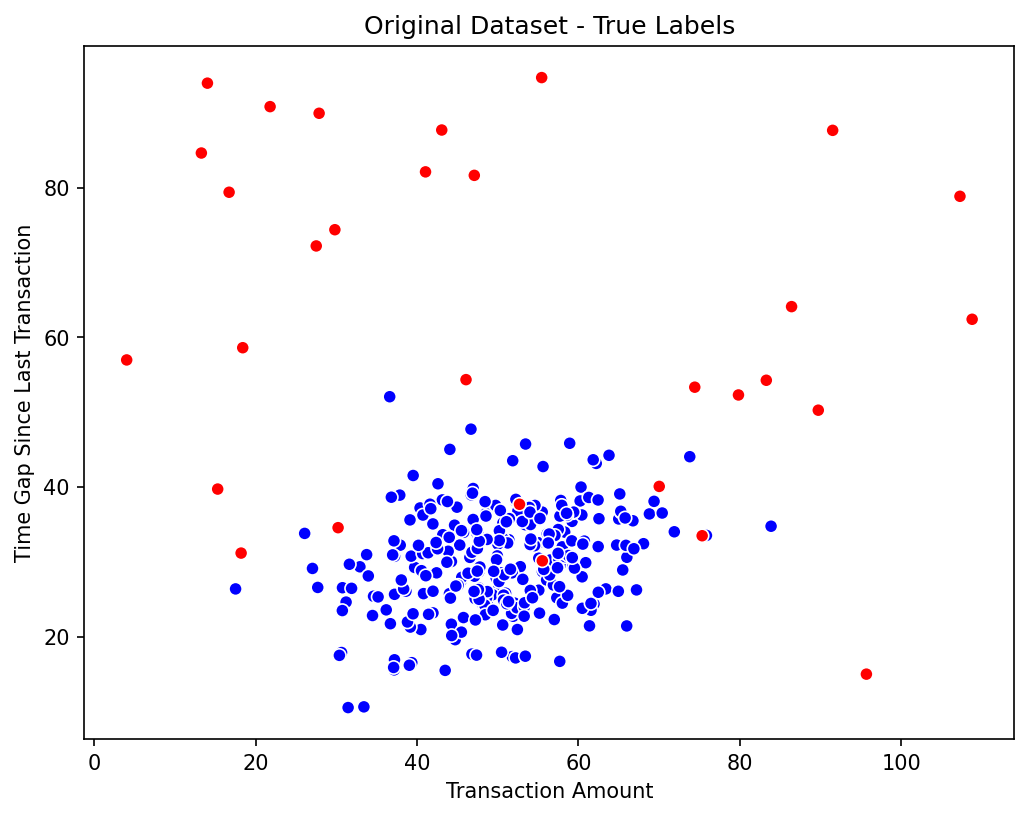
\includegraphics[width=0.85\textwidth]{plot_dataset.png}
\end{figure}

\vspace{14pt}

\begin{tcolorbox}
\textbf{Task 8: Plot Decision Boundaries}

Visualize how both methods (Isolation Forest and Gaussian) separate normal 
data from anomalies. Compare the shape of the regions produced by each method.

\begin{lstlisting}
def plot_decision_boundary(model_or_fn, X, method):
    x_min, x_max = X[:,0].min()-10, X[:,0].max()+10
    y_min, y_max = X[:,1].min()-10, X[:,1].max()+10
    xx, yy = np.meshgrid(
        np.linspace(x_min, x_max, 100),
        np.linspace(y_min, y_max, 100)
    )
    grid_pts = np.c_[xx.ravel(), yy.ravel()]

    if method == "iforest":
        Z = model_or_fn.predict(grid_pts)
    elif method == "gaussian":
        mu, sigma, thr = model_or_fn
        Z = predict_gaussian(grid_pts, mu, sigma, thr)
    else:
        return

    Z = Z.reshape(xx.shape)
    plt.contourf(xx, yy, Z, alpha=0.4,
                 colors=['#ffc2c2', '#ffffff'])
\end{lstlisting}
\end{tcolorbox}

\begin{figure}[H]
\centering
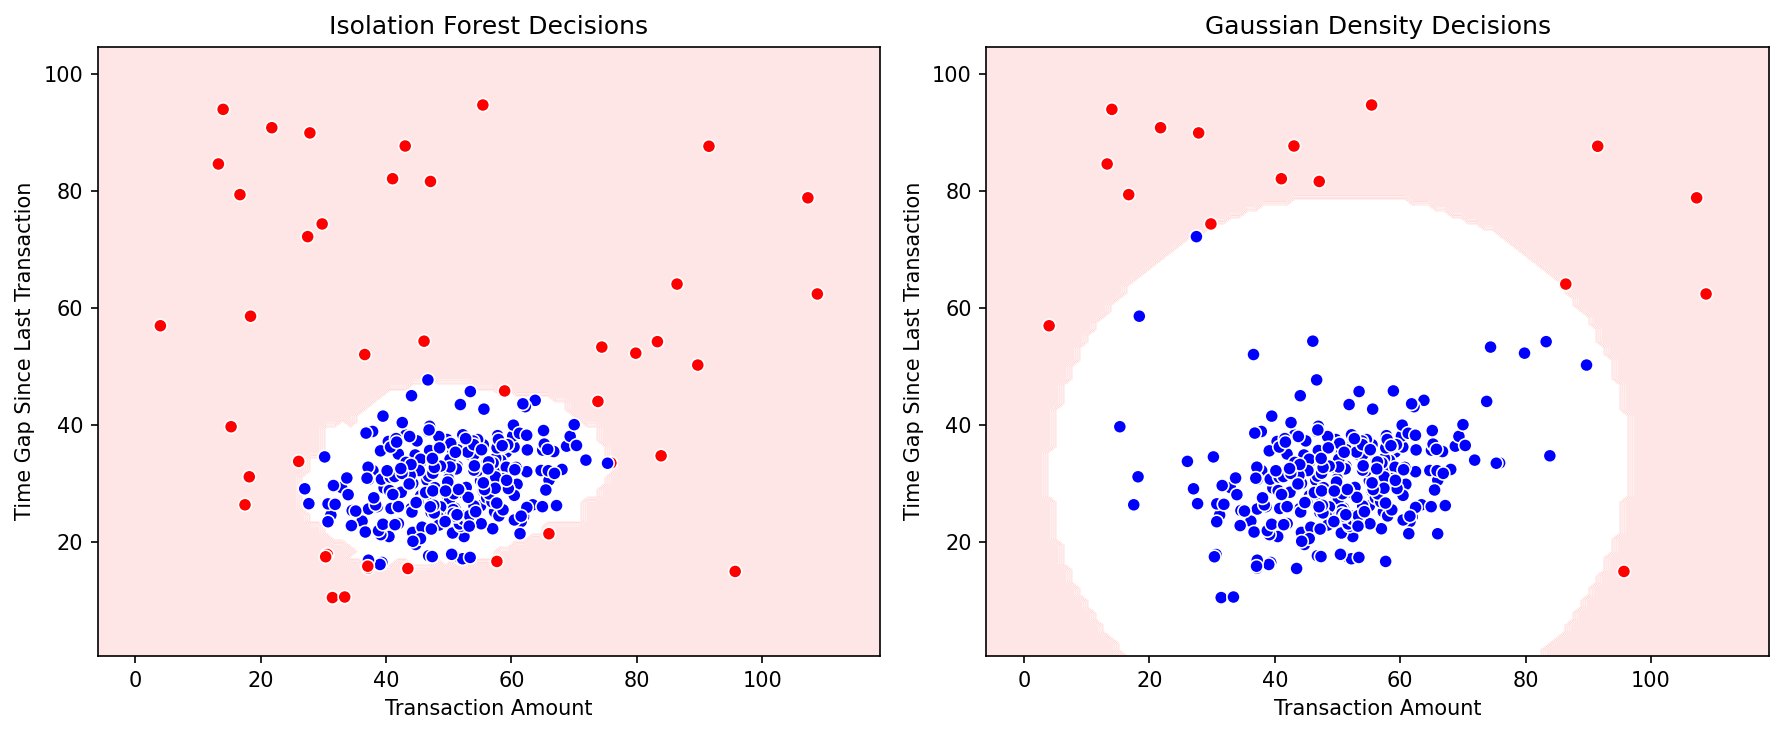
\includegraphics[width=\textwidth]{plots.png}
\end{figure}

\vspace{20pt}

\section*{Testing Results}
\begin{center}
\includegraphics[width=\textwidth]{test_results.png}
\end{center}

\end{document}